\section{Application Debugging}

\subsection{Good practices}

\begin{frame}
  \frametitle{Good practices}
  \begin{itemize}
    \item Some good practices can allow you to save time before even needing to
          use a debugger
    \item Compiler are now smart enough to detect a wide range of errors at
          compile-time using warnings
    \begin{itemize}
      \item Using \code{-Werror -Wall -Wextra} is recommended if possible to catch
            errors as early as possible
    \end{itemize}
    \item Compilers now offer static analysis capabilities
    \begin{itemize}
      \item GCC allows to do so using the \href{https://gcc.gnu.org/onlinedocs/gcc-11.1.0/gcc/Static-Analyzer-Options.html}{-fanalyzer} flag
      \item LLVM provides \href{https://clang-analyzer.llvm.org/command-line.html}{dedicated tools} that can be used in build process
    \end{itemize}
  \end{itemize}
\end{frame}

\subsection{Instrumenting code crashes}

\begin{frame}[fragile]
  \frametitle{Instrumenting code crashes}
  \begin{itemize}
      \item Displaying a backtrace from your application were the crash happened
            is useful to debug and can be done using \code{backtrace()}
            (\manpage{backtrace}{3}) GNU extension function:
  \end{itemize}
    \begin{block}{}
      \begin{minted}[fontsize=\small]{c}
char **backtrace_symbols(void *const *buffer, int size);
      \end{minted}
    \end{block}

  \begin{itemize}
    \item Thanks to \code{signal()} (\href{https://man7.org/linux/man-pages/man7/signal.7.html}{man signal(3)})
          we can add hooks on specific signals to print our backtrace
    \begin{itemize}
      \item This is for example very useful to catch \code{SIGSEGV} signal to dump our current backtrace
    \end{itemize}
    \begin{block}{}
      \begin{minted}[fontsize=\small]{c}
void (*signal(int sig, void (*func)(int)))(int);
      \end{minted}
    \end{block}
  \end{itemize}
\end{frame}

\begin{frame}[fragile]
  \frametitle{Custom code crash report}
  \begin{columns}
    \column{0.5\textwidth}
    \begin{block}{}
      \begin{minted}[fontsize=\tiny]{c}
[...]
void callee(void *ptr) {
  int *myptr = (int *)ptr;
  printf("Executing suspicious operation\n");
  myptr[2] = 0;
}

void caller(void) {
  void *ptr = NULL;
  callee(ptr);
}

void segfault_handler(int sig) {
  void *array[20];
  size_t size;

  fprintf(stderr, "Segmentation fault!\n");
  size = backtrace(array, 20);
  backtrace_symbols_fd(array, size, STDERR_FILENO);
  exit(1);
}

int main() {
  signal(SIGSEGV, segfault_handler);
  printf("Calling a faulty function\n");
  caller();
  return 0;
}
      \end{minted}
    \end{block}
    \column{0.5\textwidth}
    \begin{block}{}
      \begin{minted}[fontsize=\tiny]{console}
[root@arch-bootlin-alexis custom_backtrace]# ./main
Calling a faulty function
Executing suspicious operation
Segmentation fault!
./main(segfault_handler+0x60)[0x55c6e4c1723c]
/usr/lib/libc.so.6(+0x38f50)[0x7fecb0a95f50]
./main(callee+0x2b)[0x55c6e4c171b4]
./main(caller+0x1c)[0x55c6e4c171d9]
./main(main+0x2c)[0x55c6e4c1729a]
/usr/lib/libc.so.6(+0x23790)[0x7fecb0a80790]
/usr/lib/libc.so.6(__libc_start_main+0x8a)[0x7fecb0a8084a]
./main(_start+0x25)[0x55c6e4c170b5]
      \end{minted}
    \end{block}
  \end{columns}
\end{frame}

\subsection{The ptrace system call}

\begin{frame}[fragile]
  \frametitle{ptrace}
  \begin{itemize}
    \item The {\em ptrace} mechanism allows processes to trace other processes by
          accessing tracee memory and register contents
    \item A tracer can observe and control the execution state of another
          process
    \item Works by attaching to a tracee process using the \code{ptrace()}
          system call (see \manpage{ptrace}{2})
    \item Can be executed directly using the \code{ptrace()} call but often used
          indirectly using other tools.

  \begin{block}{}
    \begin{minted}[fontsize=\small]{C}
long ptrace(enum __ptrace_request request, pid_t pid, void *addr, void *data);
    \end{minted}
  \end{block}

    \item Used by {\em GDB}, {\em strace} and all debugging tools that need access to the
          tracee process state
  \end{itemize}
\end{frame}

\subsection{GDB}

\begin{frame}
  \frametitle{GDB: GNU Project Debugger}
  \fontsize{11}{11}\selectfont
  \begin{columns}[T]
    \column{0.8\textwidth}
    \begin{itemize}
    \item The debugger on GNU/Linux, available for most embedded
      architectures.
    \item Supported languages: C, C++, Pascal, Objective-C, Fortran,
      Ada...
    \item Command-line interface
    \item Integration in many graphical IDEs
    \item Can be used to
      \begin{itemize}
      \item control the execution of a running program, set
        breakpoints or change internal variables
      \item to see what a program was doing when it crashed: post
        mortem analysis
      \end{itemize}
    \item \url{https://www.gnu.org/software/gdb/}
    \item \url{https://en.wikipedia.org/wiki/Gdb}
    \item New alternative: {\em lldb} (\url{https://lldb.llvm.org/})\\
      from the LLVM project.
    \end{itemize}
    \column{0.2\textwidth}
    
\includegraphics[width=0.9\textwidth]{common/gdb.png}
  \end{columns}
\end{frame}

\begin{frame}[fragile]
  \frametitle{GDB crash course (1/3)}
  \begin{itemize}
    \item GDB is used mainly to debug a process by starting it with {\em gdb}
    \begin{itemize}
      \item \code{$ gdb <program>}
    \end{itemize}
    \item GDB can also be attached to running processes using the program PID
    \begin{itemize}
      \item \code{$ gdb -p <pid>}
    \end{itemize}
    \item When using GDB to start a program, the program needs to be run with
    \begin{itemize}
      \item \code{(gdb) run [prog_arg1 [prog_arg2] ...]}
    \end{itemize}
  \end{itemize}
\end{frame}

\begin{frame}
  \frametitle{GDB crash course (2/3)}
  \small
  A few useful GDB commands
  \begin{itemize}
  \item \code{break foobar} (\code{b})\\
    Put a breakpoint at the entry of function \code{foobar()}
  \item \code{break foobar.c:42}\\
    Put a breakpoint in \code{foobar.c}, line 42
  \item \code{print var}, \code{print $reg} or \code{print task->files[0].fd} (\code{p})\\
    Print the variable \code{var}, the register \code{$reg} or a more
    complicated reference. GDB can also nicely display structures with all
    their members
  \item \code{info registers}\\
    Display architecture registers
  \end{itemize}
\end{frame}

\begin{frame}
  \frametitle{GDB crash course (3/3)}
  \small
  \begin{itemize}
  \item \code{continue} (\code{c})\\
    Continue the execution after a breakpoint
  \item \code{next} (\code{n})\\
    Continue to the next line, stepping over function calls
  \item \code{step} (\code{s})\\
    Continue to the next line, entering into subfunctions
  \item \code{stepi} (\code{si})\\
    Continue to the next instruction
  \item \code{finish}\\
    Execute up to function return
  \item \code{backtrace} (\code{bt})\\
    Display the program stack
  \end{itemize}
\end{frame}

\ifthenelse{\equal{\training}{debugging}}
{
\begin{frame}
  \frametitle{GDB advanced commands (1/3)}
  \small
  \begin{itemize}
    \item \code{info threads} (\code{i threads})\\
      Display the list of threads that are available
    \item \code{info breakpoints} (\code{i b})\\
      Display the list of breakpoints/watchpoints
    \item \code{delete <n>} (\code{d <n>})\\
      Delete breakpoint <n>
    \item \code{thread <n>} (\code{t <n>})\\
      Select thread number <n>
    \item \code{frame <n>} (\code{f <n>})\\
      Select a specific frame from the backtrace, the number being the one
      displayed when using \code{backtrace} at the beginning of each line
  \end{itemize}
\end{frame}

\begin{frame}
  \frametitle{GDB advanced commands (2/3)}
  \small
  \begin{itemize}
    \item \code{watch <variable>} or \code{watch \*<address>}\\
      Add a watchpoint on a specific variable/address.
    \item \code{print variable = value} (\code{p variable = value})\\
      Modify the content of the specified variable with a new value
    \item \code{break if condition == value}\\
      Break only if the specified condition is true
    \item \code{watch if condition == value}\\
      Trigger the watchpoint only if the specified condition is true
    \item \code{x/<n><u> <address>}\\
      Display memory at the provided address. \code{n} is the amount of memory to
      display, \code{u} is the type of data to be displayed (\code{b/h/w/g}).
      Instructions can be displayed using the \code{i} type.
  \end{itemize}
\end{frame}

\begin{frame}
  \frametitle{GDB advanced commands (3/3)}
  \small
  \begin{itemize}
    \item \code{list <expr>}\\
      Display the source code associated to the current program counter location.
    \item \code{disassemble <location,start_offset,end_offset>} (\code{disas})\\
      Display the assembly code that is currently executed.
    \item \code{p function(arguments)}\\
      Execute a function using GDB. NOTE: be careful of any side effects that
      may happen when executing the function
    \item \code{p $newvar = value}\\
      Declare a new gdb variable that can be used locally or in command sequence
    \item \code{define <command_name>}\\
      Define a new command sequence. GDB will prompt for the sequence of
      commands.
  \end{itemize}
\end{frame}
}
{
\subsection{Remote debugging}
}

\begin{frame}
  \frametitle{Remote debugging}
  \begin{itemize}
  \item In a non-embedded environment, debugging takes place using \code{gdb}
    or one of its front-ends.
  \item \code{gdb} has direct access to the binary and libraries compiled
    with debugging symbols.
  \item However, in an embedded context, the target platform
    environment is often too limited to allow direct debugging with
    \code{gdb} (2.4 MB on x86).
  \item Remote debugging is preferred
    \begin{itemize}
    \item \code{ARCH-linux-gdb} is used on the development workstation, offering
      all its features.
    \item \code{gdbserver} is used on the target system (only 400 KB
      on arm).
    \end{itemize}
  \end{itemize}
  \begin{center}
    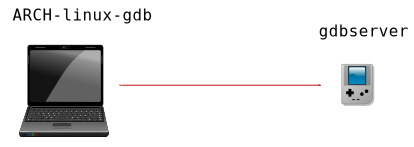
\includegraphics[width=0.5\textwidth]{common/gdb-vs-gdbserver.pdf}
  \end{center}
\end{frame}

\begin{frame}
  \frametitle{Remote debugging: architecture}
  \begin{center}
    \includegraphics[width=\textwidth]{common/gdb-vs-gdbserver-architecture.pdf}
  \end{center}
\end{frame}

\begin{frame}
  \frametitle{Remote debugging: usage}
  \begin{itemize}
  \item On the target, run a program through \code{gdbserver}.\\
    Program execution will not start immediately.\\
    \code{gdbserver :<port> <executable> <args>}
    \code{gdbserver /dev/ttyS0 <executable> <args>}
  \item Otherwise, attach \code{gdbserver} to an already running program:\\
    \code{gdbserver --attach :<port> <pid>}
  \item Then, on the host, start \code{ARCH-linux-gdb <executable>},\\
    and use the following \code{gdb} commands:
    \begin{itemize}
    \item To tell \code{gdb} where shared libraries are:\\
      \code{gdb> set sysroot <library-path>} (typically path to build space without \code{lib/})
    \item To connect to the target:\\
      \code{gdb> target remote <ip-addr>:<port>} (networking)\\
      \code{gdb> target remote /dev/ttyUSB0} (serial link)
    \end{itemize}
  \end{itemize}
\end{frame}

\begin{frame}
  \frametitle{Coredumps for post mortem analysis}
  \begin{itemize}
  \item When an application crashes due to a {\em segmentation fault}
    and the application was not under control of a debugger, we get no
    information about the crash
  \item Fortunately, Linux can generate a \code{core} file that
    contains the image of the application memory at the moment of the
    crash in the ELF format. gdb can use this \code{core} file to let
    us analyze the state of the crashed application
  \item On the target
    \begin{itemize}
    \item Use \code{ulimit -c unlimited} in the shell starting the
      application, to enable the generation of a \code{core} file
      when a crash occurs
    \item The output name for the coredump file can be modified using
      \code{/proc/sys/kernel/core_pattern}.
    \item See \manpage{core}{5}
    \end{itemize}
  \item On the host
    \begin{itemize}
    \item After the crash, transfer the \code{core} file from the target to
      the host, and run
      \code{ARCH-linux-gdb -c core-file application-binary}
    \end{itemize}
  \end{itemize}
\end{frame}

\begin{frame}
  \frametitle{minicoredumper}
  \begin{itemize}
  \item Coredumps can be huge for complex applications
  \item minicoredumper is a userspace tool based on the standard core dump
    feature
    \begin{itemize}
    \item Based on the possibility to redirect the core dump output to a
      user space program via a pipe
    \end{itemize}
  \item Based on a JSON configuration file, it can:
    \begin{itemize}
    \item save only the relevant sections (stack, heap, selected ELF
      sections)
    \item compress the output file
    \item save additional information from \code{/proc}
    \end{itemize}
  \item \url{https://github.com/diamon/minicoredumper}
  \item ``Efficient and Practical Capturing of Crash Data on Embedded
    Systems''
    \begin{itemize}
      \item Presentation by minicoredumper author John Ogness
      \item Video: \url{https://www.youtube.com/watch?v=q2zmwrgLJGs}
      \item Slides:
        \href{https://elinux.org/images/8/81/Eoss2023_ogness_minicoredumper.pdf}
             {elinux.org/images/8/81/Eoss2023\_ogness\_minicoredumper.pdf}
    \end{itemize}
  \end{itemize}
\end{frame}


\begin{frame}
  \frametitle{GDB: going further}
  \begin{itemize}
    \item Tutorial: Debugging Embedded Devices using GDB - Chris Simmonds, 2020
    \begin{itemize}
      \item Slides: \url{https://elinux.org/images/0/01/Debugging-with-gdb-csimmonds-elce-2020.pdf}
      \item Video: \url{https://www.youtube.com/watch?v=JGhAgd2a_Ck}
    \end{itemize}
  \end{itemize}
  \begin{center}
    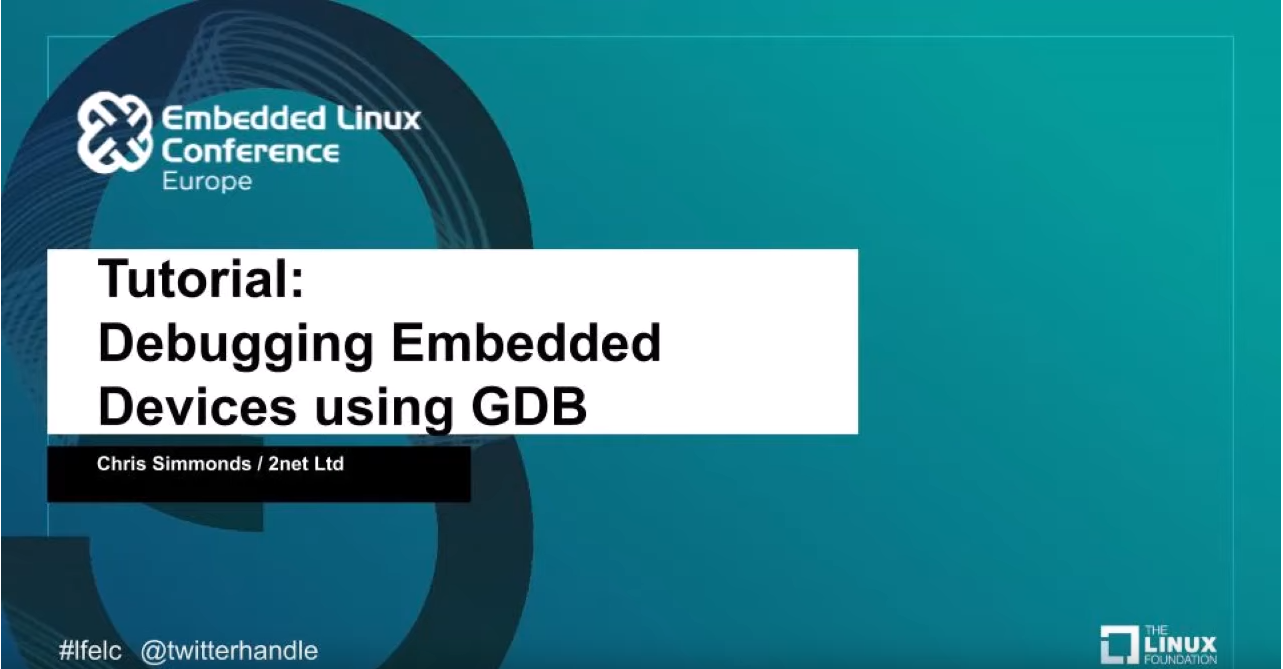
\includegraphics[height=0.6\textheight]{slides/debugging-application-debugging/gdb_tuto_elce_2020.png}
  \end{center}
\end{frame}

\begin{frame}
  \frametitle{GDB Python Extension}
  \begin{itemize}
    \item GDB features a \href{https://sourceware.org/gdb/onlinedocs/gdb/Python.html}{python integration},
          allowing to script some debugging operations
    \item When executing python under GDB, a module named {\em gdb} is available
          and all the GDB specific classes are accessible under this module
    \item Allows to add new types of commands, breakpoint, printers
    \begin{itemize}
      \item Used by the kernel to create new commands with the python GDB scripts
    \end{itemize}
    \item Allows full control and observability over the debugged program using
          GDB capabilities from Python scripts
    \begin{itemize}
      \item Controlling execution, adding breakpoints, watchpoints, etc
      \item Accessing the process memory, frames, symbols, etc
    \end{itemize}
  \end{itemize}
  \begin{center}
    
\includegraphics[height=0.2\textheight]{slides/debugging-application-debugging/python_logo.pdf}
  \end{center}
\end{frame}

\begin{frame}[fragile]
  \frametitle{GDB Python Extension (1/2)}
  \begin{block}{}
    \begin{minted}[fontsize=\tiny]{python}
class PrintOpenFD(gdb.FinishBreakpoint):
  def __init__(self, file):
    self.file = file
    super(PrintOpenFD, self).__init__()

  def stop (self):
    print ("---> File " + self.file + " opened with fd " + str(self.return_value))
    return False

class PrintOpen(gdb.Breakpoint):
  def stop(self):
    PrintOpenFD(gdb.parse_and_eval("file").string())
    return False

class TraceFDs (gdb.Command):
  def __init__(self):
    super(TraceFDs, self).__init__("tracefds", gdb.COMMAND_USER)

  def invoke(self, arg, from_tty):
    print("Hooking open() with custom breakpoint")
    PrintOpen("open")

TraceFDs()
    \end{minted}
  \end{block}
\end{frame}

\begin{frame}[fragile]
  \frametitle{GDB Python Extension (2/2)}
  \begin{itemize}
    \item Python scripts can be loaded using gdb \code{source} command
    \begin{itemize}
      \item Or the script can be named <program>-gdb.py and will be loaded automatically by GDB
    \end{itemize}
  \end{itemize}
  \begin{block}{}
    \begin{minted}[fontsize=\small]{console}
(gdb) source trace_fds.py 
(gdb) tracefds 
Hooking open() with custom breakpoint
Breakpoint 1 at 0x33e0
(gdb) run
Starting program: /usr/bin/touch foo bar
Temporary breakpoint 2 at 0x5555555587da
---> File foo opened with fd 3
Temporary breakpoint 3 at 0x5555555587da
---> File bar opened with fd 0
    \end{minted}
  \end{block}
\end{frame}

\begin{frame}[fragile]
  \frametitle{Common debugging issues}
  \begin{itemize}
    \item You will likely encounter some issues while debugging, like poor address->symbols conversion, "optimized out" values or functions, empty backtraces...
    \item A quick checklist before starting debugging can spare you some troubles:
    \begin{itemize}
      \item Make sure your host binary has \href{https://gcc.gnu.org/onlinedocs/gcc/Debugging-Options.html}{debug symbols}: with gcc, ensure \code{-g} is provided, and use non-stripped version with host gdb
      \item Disable \href {https://gcc.gnu.org/onlinedocs/gcc-4.9.2/gcc/Optimize-Options.html}{optimizations} on final binary (\code{-O0}) if possible, or at least use a less intrusive level (\code{-Og})
      \begin {itemize}
        \item Static functions can for example be folded into caller depending on the optimization level, so they would be missing from backtraces
    \end{itemize}
      \item Prevent code optimization from reusing frame pointer register: with GCC, make sure \code {-fno-omit-frame-pointer} option is set
        \begin{itemize}
          \item Not only true for debugging: any profiling/tracing tool relying on backtraces will benefit from it
        \end{itemize}
    \end{itemize}
    \item Your application is probably composed of multiple libraries: you will need to apply those configurations on all used components!
  \end{itemize}
\end{frame}

\setuplabframe
{Solving an application crash}
{
  Debugging an application crash
  \begin{itemize}
    \item Code generation analysis with compiler-explorer
    \item Using GDB and its Python support
    \item Analyzing and using a coredump
  \end{itemize}
}
